%TODO Programación y configuración de la interfaz Cypress 
	Como interfaz entre la FPGA y la PC se utilizó la placa de desarrollo CY3684 FX2LP EZ-USB Development Kit de Cypress Semiconductor. Esta placa posee como núcleo un CY7C68013A, circuito integrado que posee todas las herramientas necesarias para realizar la interfaz, como así también un buen número de periféricos que permiten al desarrollador realizar pruebas y depuración.\\
	
	Entre estas, se pueden mencionar 6 pulsadores, de los cuales cuatro se utilizan para proposito general, uno para reestablecer los valores por defecto de la placa y uno para enviar señales de suspensión y reestablecimiento del programa actualmente cargado en el microcontrolador. A su vez, posee dos memorias EEPROM que sirven para cargar firmware y archivos de configuración del sistema, un display de 8 segmentos, 4 leds de multiple propósito, dos puertos UART, una salida de pines compatible con puertos ATA y 6 puertos de 20 pines que se utilizan para la conexión hacia el chip núcleo. Como soporte para el firmware, posee también un bloque de \SI{64}{\kilo\byte} de memoria SRAM.\\
	
	Se seleccionó este controlador como interfaz con el objetivo de utilizar la m9enor cantidad de los recursos configurables de la FPGA, de forma tal que estos queden disponibles para el desarrollo de los sistemas que necesiten los potenciales sensores que se desee leer a posteriori.\\
	
	A continuación se describe en datalle la arquitectura y las funciones del CI CY7C68103A, la configuración de funcinamiento escogida, y el desarrollo del firmaware en base al framwork provisto por Cypress que facilita la implementación de periféricos.\\
	
	\section{Arquitectura y Funciones del CY7C68013A}
	El núcleo del Kit de Desarrollo FX2LP EZ-USB es un CY7C68013A. Dicho circuito integrado, cuya arquitectura se presenta en la Figura \ref{arqEzUSB}. Los chips de la familia FX2LP integran un transceptor USB, un SIE {\it Serial Interfaz Engine}, buffers de datos, un microcontrolador 8051 mejorado y una interfaz programable hacia los periféricos. Además posee un un PLL y un divisor configurable a través de los cuales provee al sistema de una señal de reloj adecuada para el correcto funcionamiento del sistema.\\
	
	\begin{figure}
		\centering
		%TODO meter la imagen
		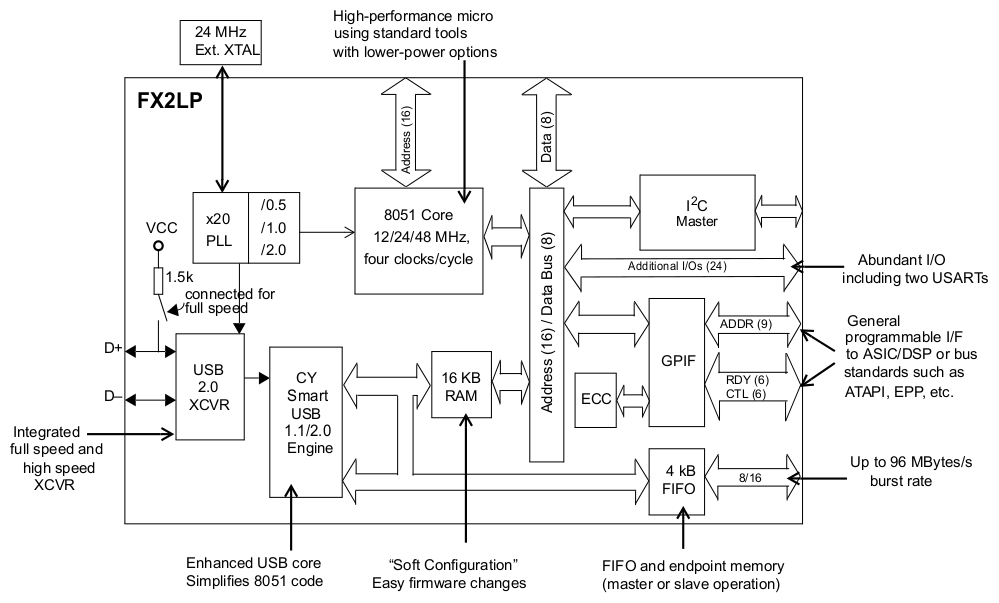
\includegraphics[width = 0.5*\textwidth]{arqfx2lp.png}
		%TODO Meter la referencia
		\caption{Arquitectura FX2LP} 
		\label{arqExUSB}
	\end{figure}

	La arquitectura que posee el integrado permite al usuario trasmitir datos desde y hacia la PC de diversas formas
\section{Programación y Configuración de la Interface}



%
%	%TODO Elección de la configuración de la interfaz Cypress para cumplir con los requerimientos del sistema
%	El objetivo que persigue el diseño de sensores es transformar alguna variable física en una señal diferente que luego pueda ser medida y registrada.Esto dá lugar a lo que se conoce
%como dato. Un dato es, entonces, el valor de una medida que representa la variable física que se desea conocer.\\
%	Sin embargo, los datos aislados por sí mismos dicen muy poco con respecto a la variable medida. Para que un dato sea realmente útil, al mismo se le debe aplicar una serie de metodos
%y procedimientos que otorguen información.\\
%	La información es el resultado de la comparación de un conjunto de datos entre sí, de manera que permita encontrar relaciones entre ellos. Con la información, un repector aumenta el
%conocimiento que posee en relación al sistema medido.\\
%	En otras palabras para adquirir conocimiento, es necesario obtener información; para adquirir información es necesario contar con un conjunto de datos que permitan ser procesados;
%a su vez, los datos son obtenidos por sensores.\\
%	Como ejemplo de lo anterior, el lector puede imaginar que se desea conocer la presión dentro de un recipiente. Para ello, uno coloca un manómetro como sensor. El manómetro posee un
%transductor que transforma la presión en desplazamiento, exhibido al usuario a través de una aguja. El usuarió bien podría registrar solo la distancia que la aguja fue movida. Sin embargo,
%este dato por si solo, no arroja ningún tipo de conocimiento sobre la presión interior, sino hasta que se compare ese desplazamiento con algún desplazamiento conocido, que tal vez
%el fabricante del manómetro, el cual hay acolocado una escala graduada en el mismo, o bien el usuario mismo haya medido con anterioridad y calibardo el manómetro, de forma tal que la lectura
%resulte útil. en este ejmplo, entonces, el que desee conocer la presión en el interior del recipiente, debe ser capaz de medir el desplazamiento de la aguja del manómetro y a su vez, debe conocer
%el valor de referencia que permita comparar y obtener información de dicho sensor.\\
%	El ejemlo de anterior, brinda una cuestión útil al objetivo de este trabajo. El procesamiento de los datos se puede realizar in situ, es decir, en el momento de realizar la medida, como
%en el caso de la escala graduada colocada por el fabricante; o a posteriori, cuando el usuario mide el desplazamiento y luego lo compara con valores patrones que tomó anteriormente como referencia.
%En ambos casos, el elemento común es el dato almacenado previamente, es decir, el dato conocido, ya sea en la escala graduada, como así también en los apuntes, tablas o cualquier otra fuente
%en la que el usuario pudo registrar los valores de referencia.\\
%	Se resalta aquí la necesidad de almacenar datos para proceder luego a la etapa de procesamiento y obtención de información. En sistemas digitales, este almacenamiento puede darse en diversas
%formas y etapas. En un primer momento, los datos poueden ser almacenados en un circuito específico diseñado para obtener los datos directamente desde el sensor. Si bien esto es lo ideal en cuanto a
%velocidad, puede llegar a ser costoso y, a su vez, limitado en cantidad de almacenamiento. Es por esto que puede ser volcado en otros sistemas de almacenamiento, tales como cintas magnéticas, 
%memorias flash, etc. Sin embargo, esto requiere mas recursos y, dependiendo la aplicación, puede llegar a ser limitado en capcidad. Entonces, se plantea como solución a esto, transmitir la información
%a una PC, que con las características modernas pueden tener tanto espacio como sea necesario y a su vez, se puede preparar de forma tal que se encuentre lista para el mejor procesador de datos
%conocido hasta la fecha (EXCEL :P).
%	La ejor forma de transmitir datos desde o hasta una pc, en cuanto a disponibilidad se refiere, es el USB.
%	La versión 2.0 de USB fue desarrollada para lograr una mejor tasa de datos, que permita la adquisición de imagenes a través de lo que en su momento se empezaba a utilizar, las camaras
%web.
%	Para ello, la mejor configuración que ofrece el standar es a través de la comunicación isocrónica, o tambien conocida como streaming. Esta configuración optimiza el ancho de banda disponible
%en el protocolo usb, alcanzando una tasa de bits utiles de hasta [ver en las especs].
%	Por esto, se configuro la CY-IF de forma tal que los datos que provengan desde la FPGA, que es en dnd se implementaran los sensores, hasta la PC de forma iscorónica.
%	En el sentido inverso se supone que solo se transmitiran comandos de control que el sistema debera manejar. Al enviar menos datos, se configuro la salida de la PC con la comunicación 
%estandar diseñada en USB, es decir, la comunicaciójn por bultos.
%
%	La comunicación USB es un sistema conocido como maestro-esclavo, en donde un sistema central cemite comandos o directivas hacia sus esclavos y en funicón de esto los esclavos responden
%a la solicitud del maestro. En usb el maestro es siempre el PC y los dispositivos en ella conectada son los esclavos. la pc, entonces, solicita a cada uno de sus esclavos los datos que posea.
%Es por esto que los diseñadores de cypress previeron que podría existir un cuello de botella entre la generación de datos y lo que solitica la PC. Para ello colocaron en la configuración interna
%del chip buffers configurables que pueden ser asignado a cualquiera de los enpojints de entrada o salida.
%inicialmente cada uno puede tener un mininmo de dos buffers y dependiendo de las necesdades del sistema, hasta cuatro buffers.
%	Para ello, se prevee que los dipositivos que más datos generen tengan mayor capacidad que los que menos datos generan. por eso, se configuro la entrada a la computadora de forma que tenga
%una mayor cantidad de buffers. La mayor posibilidad soportada por es de 3 buffers de 1024 bytes cada uno, es decir, un total de 3072 bytes. a la entrada se utilzó elresto de lso buffer disponibles
%es decir, posee solo dos buffers de 512 bytes, es decir, un total de 1024 bytes en simultaneo.
%	
%	Para la configuración de la CY-IF, existe un \it{framework} provisto por el fabricante, escrito en C que maneja los distintos módulos del kit de desarrollo.
%
%
%
%
%
% 
%	Una vez adquirido un dato, el mismo debe ser almacenado en forma segura, de forma tal que, una vez obtenida una cantidad suficiente que permita extraer información, pueda ser procesada.
%	El proceso de los datos puede swer realizado in situ o a posteriori.
%	Cada uno de ellos presenta ventajas e inconvenientes
%	entre las ventajas de el procesamiento de datos in situ, es que la información se obtiene de una forma mucho más veloz. La desventaja es que el sistema desarrollado 
%Este proceso puede ser in situ, es decir, en el mismo
%momento en que los datos son adquiridos, o bien, puede hacerse a posteriori, ya sea de forma automática o manual. 
	%TODO Descripción del Framework Cypress
	%TODO Adaptación del framework para su utilización en sistemas de código abierto
	%TODO Configuración del microprocesador 8051

